	\documentclass{../preamble}
	
	% Title information
	\date{14.12.2020 - 18.12.2020}
	\sheetnumber{5}
	\version{28. Dezember 2020}
	
	% Document
	\begin{document}
	
	\maketitle
	
	\makedisclaimer
	
	\clearpage
	
	\setcounter{task}{1}
	
	\begin{tcolorbox}
	    Denken Sie an Vertrag und drei Tests bei jeder Funktion.
	\end{tcolorbox}
	
	\begin{task}[credit = \stars{0}{3}]{Temperaturumrechnung}
	    Im angloamerikanischen Maßsystem wird die Temperatur nicht wie hierzulande in Grad Celsius gemessen, sondern in Grad Fahrenheit. Da Sie damit nichts anfangen können, wollen Sie sich nun eine Funktion \code{fahr->cel} definieren, welche die aktuelle Temperatur in Grad Fahrenheit übergeben bekommt und in Grad Celsius umwandelt.
	    \br
	    \textbf{Hinweis:} Für eine gegebene Temperatur \(T_F\) in Grad Fahrenheit berechnet sich die dazugehörige Temperatur \(T_C\) in Grad Celsius über den folgenden Zusammenhang:
	    \begin{equation*}
	        T_C = (T_F - 32) \cdot \frac{5}{9}
	    \end{equation*}
	
	    \begin{solution}
	        \lstinputlisting[style = Racket]{codes/V2_Solution.rkt}
	    \end{solution}
	\end{task}
	
	\clearpage
	
	\begin{task}[credit = \stars{1}{3}]{Volumen eines Tetraeders}
	    Das Tetraeder ist ein Körper mit vier dreieckigen Seitenflächen. Sein Volumen berechnet sich über die Formel \(V(a) = \frac{\sqrt{2}}{12} a^3\), wobei \(a\) hier die Länge einer Kante ist. Sie sollen in dieser Aufgabe nun eine Funktion \code{tetrahedron-volume} schreiben, die für eine übergebene Kantenlänge \(a\) das Volumen des dazugehörigen Tetraeders zurückgibt. Gehen Sie dazu in folgenden Schritten vor:
	    \begin{enumerate}
	        \item Definieren Sie eine Funktion \code{pow3}, welche einen Parameter \(x\) bekommt, und den Wert \(x^3\) zurückgibt. Erstellen Sie außerdem eine Konstante \code{k}, mit dem Wert \(\frac{\sqrt{2}}{12}\).
	        \item Nutzen Sie die zwei vorherigen Schritte, um nun die Funktion \code{tetrahedron-volume} zu definieren, welche nur einen Parameter \code{a} bekommt.
	    \end{enumerate}
	
	    \begin{solution}
	        \lstinputlisting[style = Racket]{codes/V3_Solution.rkt}
	    \end{solution}
	\end{task}
	
	\clearpage
	
	\begin{task}[credit = \stars{1}{3}]{Relative Lage zweier Kreise zueinander}
	    Wir wollen die Lage zweier Kreise zueinander bestimmen. Definieren Sie dazu eine Prozedur \code{circles-position}, welche die Zahlen \(x1, y1, r1, x2, y2, r2\) in dieser Reihenfolge entgegennimmt und einen String zurückgibt, welche die Lage der beiden Kreise zueinander beschreibt. Dabei sind \(x\) und \(y\) die Koordinaten eines Kreismittelpunktes und \(r\) der Radius des Kreises.
	    \br
	    Zurückgegeben werden soll \code{\grqq Intersect\grqq} bei einem Schnitt der beiden Kreise, \code{\grqq External\grqq} bei keinerlei Überlappung oder \code{\grqq Interior\grqq} wenn einer der beiden Kreise vollständig im anderen liegt. Eine Berührung der beiden Kreise, egal ob von innen oder von außen, soll als Schnitt der beiden Kreise erkannt werden.
	    \br
	    Zum besseren Verständnis finden Sie im Anschluss an die Aufgabe ein Beispiel und die mathematische Konkretisierung des  Sachverhalts (dabei steht \code{d} für den Abstand der Mittelpunkte). Bei den Kreisen \(K_1\) und \(K_2\) im Beispiel sollte \code{\grqq Intersect\grqq}, bei den Kreisen \(K_1\) und \(K_3\) sollte \code{\grqq External\grqq} und bei den Kreisen \(K_2\) und \(K_3\) sollte \code{\grqq Interior\grqq} zurückgegeben werden.
	
	    \begin{minipage}{0.45 \linewidth}
	    	\begin{figure}[H]
	    		        \centering
	        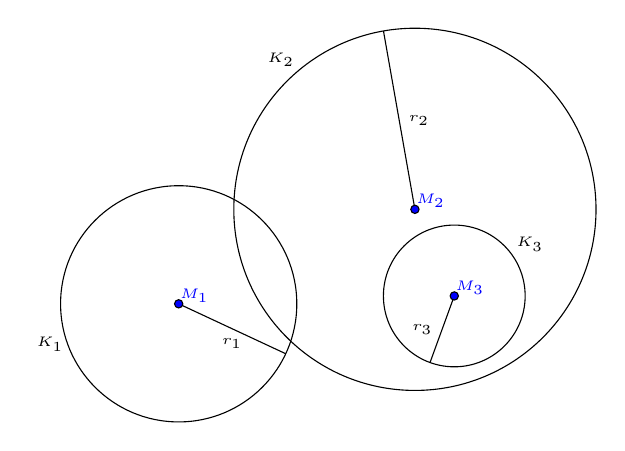
\begin{tikzpicture}[
		        every node/.style = {
		        	font = \tiny
		        },
		        center/.style = {
		        draw = black,
		        fill = blue,
		        minimum size = 3pt,
		        thin,
		        circle,
		        inner sep = 0pt,
		        label = {[blue, label distance = -6pt]above right:#1}
		    }]
		    	\draw (0, 0) circle (1.5cm) node[center = $M_{1}$] {} -- node[below] {$r_{1}$} +(-25:1.5cm) +(200:1.5cm) node[left = -2pt] {$K_{1}$};
		    	\draw (3, 1.2) circle (2.3cm) node[center = $M_{2}$] {} -- node[right] {$r_{2}$} +(100:2.3cm) +(130:2.3cm) node[above left = -2pt] {$K_{2}$};
		    	\draw (3.5, 0.1) circle (0.9cm) node[center = $M_{3}$] {} -- node[left] {$r_{3}$} +(-110:0.9cm) +(35:0.9cm) node[above right = -2pt] {$K_{3}$};
	\end{tikzpicture}
	    	\end{figure}
	    \end{minipage}
	    \begin{minipage}{0.45 \linewidth}
	        \begin{equation*}
	            \text{circles-position} =
	            \begin{cases}
	                \text{Interior}  & \text{if } d < \vert r_1 - r_2 \vert
	                \\
	                \text{External}  & \text{if } r_1 + r_2 < d
	                \\
	                \text{Intersect} & \text{otherwise}
	            \end{cases}
	        \end{equation*}
	    \end{minipage}
	
	    Zur Berechnung von \code{d} verwenden Sie den euklidischen Abstand der Mittelpunkte der zwei zu vergleichenden Kreise. Der Abstand zweier Punkt \(p_1 = (x_1, y_1)\) und \(p_2 = (x_2, y_2)\) ist folgendermaßen definiert \(d_{p_1, p_2} = \sqrt{(x_2 - x_1)^2 + (y_2 - y_1)^2}\)
	
	    \clearpage
	
	    \begin{solution}
	        \lstinputlisting[style = Racket]{codes/V4_Solution.rkt}
	    \end{solution}
	\end{task}
	
	\clearpage
	
	\begin{task}[credit = \stars{1}{3}]{Euklidischer Algorithmus}
	    In der folgenden Aufgabe soll das Konzept der Rekursion verinnerlicht werden. Dazu werfen wir einen Blick auf eine Version des euklidischen Algorithmus, welcher Ihnen vielleicht schon aus der Mathematik bekannt ist. Für zwei natürliche Zahlen \(a\)und \(b\) lässt sich mit ihm der größte gemeinsame Teiler der beiden Zahlen berechnen. Dabei geht der Algorithmus wie folgt vor:
	    \br
	    Gilt \(b = 0\) so wird \(a\) zurückgegeben, ist hingegen \(a = 0\) so wird \(b\) zurückgegeben. Gilt \(a > b\) so wird der Algorithmus mit einem neuen \(\hat{a} = a - b\) und dem \grqq alten\grqq{} \(b\) aufgerufen. Im anderen Fall wird der Algorithmus mit dem \grqq alten\grqq{} \(a\) und einem neuen \(\hat{b} = b - a\) aufgerufen. Definieren Sie eine Prozedur \code{(euclid a b)}, welche diese Version des euklidischen Algorithmus rekursiv umsetzt.
	
	    \begin{solution}
	        \lstinputlisting[style = Racket]{codes/V5_Solution.rkt}
	    \end{solution}
	\end{task}
	
	\clearpage
	
	\begin{task}[credit = \stars{1}{3}]{Listenausdrücke auswerten}
	    {\large\textbf{Teil A:}} Werden die folgenden Ausdrücke ohne Fehler durch Racket ausgeführt? Falls nein, begründen Sie wo und warum es zu Problemen kommt.
	    \begin{enumerate}
	        \item (\textcolor{keywordcolor}{cons} 1 (\textcolor{keywordcolor}{cons} 2 (\textcolor{keywordcolor}{cons} 3)))
	        \item (\textcolor{keywordcolor}{cons} 1 (\textcolor{keywordcolor}{list} 2 (\textcolor{keywordcolor}{list} (\textcolor{keywordcolor}{list} 3 + 4))))
	        \item (\textcolor{keywordcolor}{list} (\textcolor{keywordcolor}{cons} \textcolor{keywordcolor}{empty} 1)(\textcolor{keywordcolor}{cons} 2 \textcolor{keywordcolor}{empty})(\textcolor{keywordcolor}{cons} 3 \textcolor{keywordcolor}{empty}))
	        \item (\textcolor{keywordcolor}{first} \textcolor{keywordcolor}{empty})
	    \end{enumerate}
	    {\large\textbf{Teil B:}} Liefern die folgenden Listenausdrücke dasselbe Ergebnis zurück?
	    \begin{enumerate}
	        \item (\textcolor{keywordcolor}{cons} 1 (\textcolor{keywordcolor}{cons} 2 (\textcolor{keywordcolor}{cons} 3 \textcolor{keywordcolor}{empty}))) und (\textcolor{keywordcolor}{list} 1 2 3 \textcolor{keywordcolor}{empty})
	        \item (\textcolor{keywordcolor}{cons} (\textcolor{keywordcolor}{list} \grqq(\textcolor{keywordcolor}{list} )\grqq)\textcolor{keywordcolor}{empty}) und (\textcolor{keywordcolor}{list} \grqq\textcolor{keywordcolor}{list}\grqq{} \textcolor{keywordcolor}{empty})
	        \item (\textcolor{keywordcolor}{list} 7 \grqq *\grqq{} 6 \grqq =\grqq{} 42) und (\textcolor{keywordcolor}{cons} 7 (\textcolor{keywordcolor}{cons} \grqq *\grqq{} (\textcolor{keywordcolor}{cons} 6 (\textcolor{keywordcolor}{cons} \grqq =\grqq{} (\textcolor{keywordcolor}{list} 42)))))
	    \end{enumerate}
	    {\large\textbf{Teil C:}} Gehen Sie nun von folgendem Codeschnipsel aus:
	    \lstinputlisting[style = Racket]{codes/V6_Task.rkt}
	    Was liefern die folgenden Aufrufe zurück?
	    \begin{enumerate}
	        \item (\textcolor{keywordcolor}{first} (\textcolor{keywordcolor}{rest} A))
	        \item (\textcolor{keywordcolor}{rest} (\textcolor{keywordcolor}{first} A))
	        \item (\textcolor{keywordcolor}{append} (\textcolor{keywordcolor}{first} B)(\textcolor{keywordcolor}{rest} (\textcolor{keywordcolor}{rest} A))(\textcolor{keywordcolor}{first} A))
	    \end{enumerate}
	
	    \begin{solution}
	        {\large\textbf{Teil A:}}
	        \begin{enumerate}
	            \item Der Ausdruck ist falsch, da \textcolor{keywordcolor}{cons} als 2. Argument immer eine Liste erwartet.
	            \item Der Ausdruck ist korrekt.
	            \item Der Ausdruck ist falsch, da \textcolor{keywordcolor}{cons} als 2. Argument immer eine Liste erwartet.
	            \item Der Ausdruck ist falsch, da \textcolor{keywordcolor}{first} eine nichtleere Liste erwartet.
	        \end{enumerate}
	        {\large\textbf{Teil B:}}
	        \begin{enumerate}
	            \item Nein, denn (\textcolor{keywordcolor}{list} 1 2 3) \(\neq\) (list 1 2 3 \textcolor{keywordcolor}{'()}).
	            \item Nein, denn (\textcolor{keywordcolor}{list} (\textcolor{keywordcolor}{list} \grqq (list )\grqq)) \(\neq\) (\textcolor{keywordcolor}{list} \grqq list\grqq{} \textcolor{keywordcolor}{'()})
	            \item Ja, denn (\textcolor{keywordcolor}{list} 7 \grqq *\grqq{} 6 \grqq =\grqq{} 42) = (\textcolor{keywordcolor}{list} 7 \grqq *\grqq{} 6 \grqq =\grqq{} 42)
	        \end{enumerate}
	        {\large\textbf{Teil C:}}
	        \begin{enumerate}
	            \item (\textcolor{keywordcolor}{list} 7)
	            \item \textcolor{keywordcolor}{'()} (leere Liste)
	            \item Es wird eine Fehlermeldung geworfen, da \code{append} als Argumente Listen erwartet. Jedoch ist das erste Argument eine Zahl.
	        \end{enumerate}
	    \end{solution}
	\end{task}
	
	\clearpage
	
	\begin{task}[credit = \stars{1}{3}]{Strukturausdrücke auswerten}
	    Gegeben sei folgende Strukturdefinition:
	    \lstinputlisting[style = Racket]{codes/V7_Task.rkt}
	    Was liefern die folgenden Aufrufe zurück?
	    \begin{enumerate}
	        \item (my-pair? (make-my-pair \grqq a\grqq{} \grqq b\grqq))
	        \item (make-my-pair 1 (make-my-pair 2 \textcolor{keywordcolor}{empty}))
	        \item (* (my-pair-two (make-my-pair 1 2))(my-pair-one (make-my-pair 3 4)))
	    \end{enumerate}
	
	    \begin{solution}
	        \begin{enumerate}
	            \item Wahr, da dies ein Struct von my-pair ist.
	            \item (make-my-pair 1 (make-my-pair 2 \textcolor{keywordcolor}{empty}))
	            \item 6
	        \end{enumerate}
	    \end{solution}
	\end{task}
	
	\begin{task}[credit = \stars{1}{3}]{Listen in Strukturen}
	    Gegeben ist ein Struct-Typ \code{abc} mit zwei Feldern \code{a} und \code{b}. Definieren Sie eine Funktion \code{foo} mit einem Parameter \code{p}. Falls \code{p} vom Typ \code{abc} und zudem der Wert im Feld \code{b} von \code{p} eine Liste ist, liefert \code{foo} eine Liste zurück, deren erstes Element der Wert von Feld \code{a} in \code{p} ist,und der Rest der zurückgelieferten Liste ist die Liste im Feld \code{b} von \code{p} (also eine Liste in der Liste). Andernfalls liefert \code{foo} einfach \textcolor{keywordcolor}{false} zurück.
	
	    \begin{solution}
	        \lstinputlisting[style = Racket]{codes/V8_Solution.rkt}
	    \end{solution}
	\end{task}
	
	\clearpage
	
	\begin{task}[credit = \stars{2}{3}]{Suche in Zahlenliste}
	    \label{task:V9}
	    Definieren Sie eine Funktion \code{contains-x?}. Diese bekommt eine Liste und eine Zahl übergeben und liefert genau dann \textcolor{keywordcolor}{true} zurück, wenn die übergebene  Zahl mindestens einmal in der übergebenen Liste vorkommt.
	
	    \begin{solution}
	        \lstinputlisting[style = Racket]{codes/V9_Solution.rkt}
	        
	        \paragraph{Alternative}
	        
	        Der alternative Lösungsvorschlag stammt von Kim Berninger.
	        \lstinputlisting[style = Racket]{codes/V9_Solution_Alternative.rkt}
	    \end{solution}
	\end{task}
	
	\clearpage
	
	\begin{task}[credit = \stars{2}{3}]{Duplikate in Zahlenliste}
	    \label{task:V10}
	    Definieren Sie eine Prozedur \code{duplicates?} mit einem Parameter \code{lst}, die genau  dann \textcolor{keywordcolor}{true} zurückliefert, wenn eine Zahl mehr als einmal in \code{lst} vorkommt.
	    \br
	    \textbf{Hinweis:} Können Sie hier vielleicht Ihre Funktion aus Aufgabe \hyperref[task:V9]{V9} verwenden?
	
	    \begin{solution}
	        \lstinputlisting[style = Racket]{codes/V10_Solution.rkt}
	        
	        \paragraph{Alternative}
	        
	        Der alternative Lösungsvorschlag stammt von Kim Berninger.
	        \lstinputlisting[style = Racket]{codes/V10_Solution_Alternative.rkt}
	    \end{solution}
	\end{task}
	
	\clearpage
	
	\begin{task}[credit = \stars{3}{3}]{Verschachtelte Listen}
	    Definieren Sie eine Prozedur \code{duplicates-deep?} mit einem Parameter \code{deep-lst}.  Es wird erwartet, dass \code{deep-lst} entweder eine Zahl oder eine Liste ist, deren  Elemente wiederum Zahlen oder Listen sind usw. (Liste von Listen von Zahlen). Die Prozedur \code{duplicates-deep?} soll \textcolor{keywordcolor}{true} oder \textcolor{keywordcolor}{false} zurückliefern, und zwar \textcolor{keywordcolor}{true} genau dann, wenn mindestens eine Zahl mehr als einmal vorkommt.
	    \br
	    \textbf{Hinweise:} Schreiben Sie sich eine Hilfsfunktion \code{collect} mit zwei Parametern \code{lst} und \code{oracle}. Nutzen Sie \code{oracle} als Akkumulator in dem Sie alle bereits vorgekommenen Zahlen in \code{oracle} speichern. Machen Sie also aus der verschachtelten Liste wieder eine normale Liste mithilfe von \code{collect}. Die Funktion aus  \hyperref[task:V10]{V10} kann Ihnen hier sehr hilfreich sein.
	
	    \begin{solution}
	        \lstinputlisting[style = Racket]{codes/V11_Solution.rkt}
	        
	        \clearpage
	        
	        \paragraph{Alternative}
	        
	        Der alternative Lösungsvorschlag stammt von Kim Berninger.
	        \lstinputlisting[style = Racket]{codes/V11_Solution_Alternative.rkt}
	    \end{solution}
	\end{task}
	
	\clearpage
	
	\begin{task}[credit = \stars{3}{3}]{Arithmetisches Mittel}
	    Gegeben seien folgende Strukturdefinition:
	    \lstinputlisting[style = Racket]{codes/V12_Task.rkt}
	    Eine Person hat ein Alter (als Zahl) und ein Geschlecht (als String). Ein Student wiederum besteht aus einer Person (vorheriges Struct) und einer Matrikelnummer (ein String).
	    \br
	    Definieren Sie nun eine Funktion \code{mean-of-ages}. Diese bekommt eine Liste von Studenten übergeben und gibt das arithmetische Mittel ihrer Alter zurück.
	    \br
	    \textbf{Hinweis:} Das arithmetische Mittel \(\bar{x}\) berechnen Sie für \(n\) Alter \(x_1, ..., x_n\) über:
	    \begin{equation*}
	        \bar{x} = \frac{1}{n} \sum_{i = 1}^n x_i = \frac{x_1 + ... + x_n}{n}
	    \end{equation*}
	
		\clearpage
		
	    \begin{solution}
	        \lstinputlisting[style = Racket]{codes/V12_Solution.rkt}
	    \end{solution}
	\end{task}
\end{document}
